\section{Общая характеристика работы}
\textbf{Актуальность темы исследования.} Быстрые изменения происходящие в городской среде, как следствие 
технического прогресса требуют формирования новых методов в планирования инфраструктуры города для 
организации комфортной жизни людей. Это относится, в том числе, и к организации транспортной 
инфраструктуры, в частности к построению маршрутов общественного транспорта. Несмотря на кажущуюся 
хаотичность все перемещения пассажиров, подчиняются определенным закономерностям, связанным с масштабом и 
планировкой городской среды. Для принятия обоснованных решений по планированию или изменению маршрутной 
сети города необходимо выявить закономерности поведения населения и сформировать обобщенную модель, на 
основе которой можно строить и оценивать варианты транспортной системы. Для получения эффективных 
результатов, следует осуществлять принятие решений на основе актуальных данных, отражающих предпочтения 
жителей. В рамках магистерской диссертации следует разработать метод кластеризации предпочтений жителей города по перемещению для создания сети остановочных пунктов.

\textbf{Цель и задачи работы.} Целью данной работы являлась разработка метода кластеризации географических данных с учетом рельефа местности. Для достижения 
поставленной цели решались следующие задачи:
\begin{itemize}
    \item генерация псевдореалистичных данных о перемещениях жителей;
    \item разработка метрики расстояний, учитывающей рельеф местности;
    \item модификация и использование существующих алгоритмов для кластеризации географических данных с разработанной метрикой расстояний;
    \item представление построенных кластеров на карте.
\end{itemize}

\textbf{Объектом исследования} кластеризация предпочтений жителей города по перемещению, выраженных в виде пары точек «Пункт отправления — пункт назначения», каждая из которых содержит две координаты — широту и долготу.

\textbf{Предметом исследования} является разработка и применение методов кластеризации предпочтений жителей, учитывающих элементы рельефа местности.

% TODO
\textbf{Гипотеза исследования.} Использование данных о перемещениях жителей и автоматизация построения сети остановочных пунктов и маршрутной сети позволяют построить оптимальную сеть маршрутов общественного транспорта.

% TODO
\textbf{Научная новизна} диссертационной работы обусловлена:
\begin{itemize}
    \item автоматизации процесса построения сети остановочных пунктов без участия транспортного инженера;
    \item предложении метода, основанном на использовании данных о предпочтении жителей для построения сети остановочных пунктов;
    \item разработке метода кластеризации географических точек с учетом естественных и искуственных препятствий.
\end{itemize}

% TODO
\textbf{Практическая ценность.} Данная система может быть использована:
\begin{itemize}
    \item в системах формирования сети общественного транспорта;
    \item в системах обработки географических данных.
\end{itemize}

% TODO
\textbf{Публикации.} По материалам диссертации автором опубликовано 3 работы, \ldots из которых представлены 
в рецензируемом научном журнале, входящем в перечень Высшей аттестационной комиссии. 

% TODO
\textbf{Структура и объем работы.} Диссертационная работа состоит из введения, четырех глав, заключения, 
списка использованных источников из \ldots наименований и насчитывает \ldots страниц, в том числе \ldots 
страниц основного текста, \ldots рисунков, \ldots таблиц и \ldots приложения.

\section{Основное содержание работы}
\textbf{Во введении} обосновываются выбор темы диссертационного исследования и ее актуальность, определяются 
цели и задачи работы, объект, предмет и гипотеза исследования, формулируется научная новизна.

\textbf{В первой главе} приводятся результаты исследования предметной области. Произведен анализ общего состояния существующей проблемы в кластеризации и обработке геоданных. Рассмотрена литература по современным исследованиям в данной области и методам предлагаемых в них. Следует отметить, что обработка препятствий в существующих алгоритмах не производится напрямую с географическими данными~--- данные о препятствиях рассчитываются из диаграмм Воронова и Делоне, накладывая ограничения на рассматриваемые точки; либо не рассчитываются, а обход препятствий заключается в работе алгоритма, <<предполагающего>> наличие препятствий. В результате был сделан вывод, что существующие решения не приспособлены для работы с данными, получаемых из картографических сервисов, и не могут в полной мере учитывать элементы рельефа; и, как следствие, могут применяться для формирования сети остановочных пунктов в полуавтоматическом режиме, требуя вмешательства транспортного инженера.

Для оптимизации маршрутной сети общественного транспорта необходимо проанализировать большой объем данных, характеризующих численность и мобильность населения, среднее время перемещения, расположение мест приложения труда и жилых массивов. Источниками этих данных выступают статистические сборники, выписки о численности сотрудников крупных предприятий, собираемые муниципальными предприятиями общественного транспорта, информация о количестве проданных билетах на маршрутах общественного транспорта. Для сбора данных о перемещениях жителей организуется целый комплекс мероприятий по натурному подсчету пассажиропотока в подвижном составе общественного транспорта и на остановочных пунктах существующих маршрутов, а также анкетированию жителей. Такие традиционные методы являются достаточно трудоемкими, а полученные данные не в полной мере отражают динамично меняющуюся ситуацию. В связи с этим, необходимо использовать современные технологии и новые ресурсы для получения актуальных данных о предпочтениях жителей по перемещениям в городе и интенсивности пассажиропотоков. Основываясь на современных подходах к анализу данных можно получить ценную информацию для поддержки принятия решений в процессе планирования развития транспортной системы города.

\textbf{Во второй главе} рассмотрены и проанализированы существующие методы, применимые к задаче кластеризации географических точек, а также разработаны методы на их основе для формирования сети остановочных пунктов используя данные о предпочтениях по перемещению жителей в городе.

Пусть \( X \)~--- входная выборка точек, полученная из географических сервисов, \( k \)~--- ожидаемое число узлов (остановочных пунктов) во входной выборке. Требуется построить \( C \)~--- сеть из \( k \) остановочных пунктов, оптимальным образом охватывающие все точки из входной выборки \( X \).

\begin{figure}[b!]
    \centering
    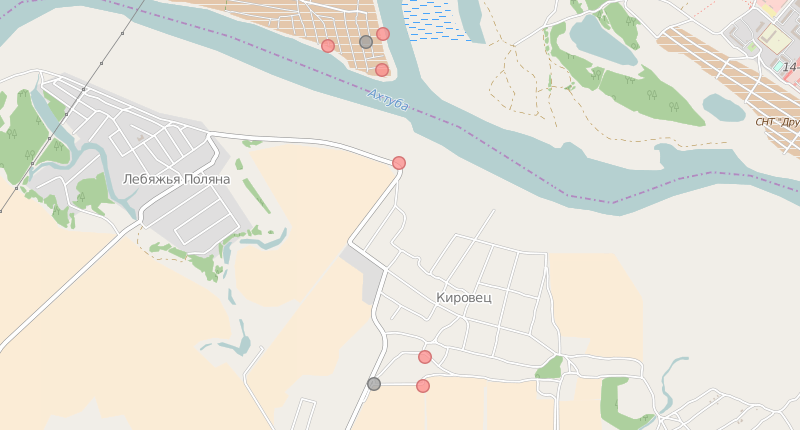
\includegraphics[width=.7\textwidth]{test_river}\\[1ex]
    \parbox{.7\textwidth}{\caption{Тестовый пример <<Река>>. Красные точки обозначают объекты выборки, черные~--- начальные центры кластеров} \label{img:river}}
    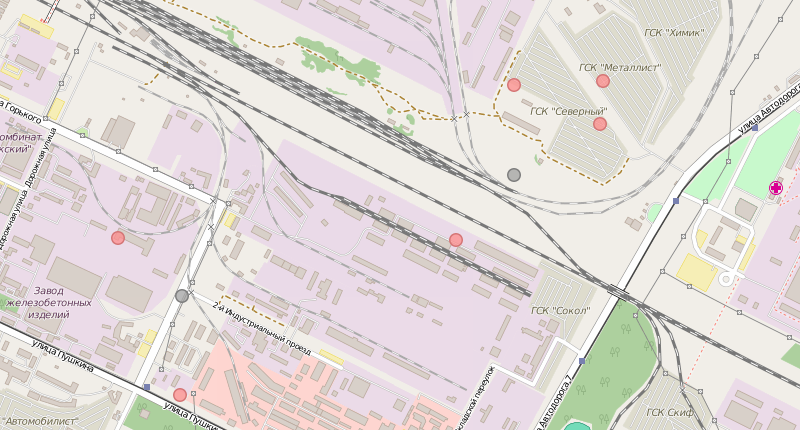
\includegraphics[width=.7\textwidth]{test_railway}\\[1ex]
    \parbox{.7\textwidth}{\caption{Тестовый пример <<Железная дорога>>. Красные точки обозначают объекты выборки, черные~--- начальные центры кластеров} \label{img:railway}}
\end{figure}

Задача является задачей кластеризации~--- машинного обучения без учителя~--- но имеет некоторые специфические особенности. Во-первых, необходимо учитывать естественные и искусственные препятствия: реки, овраги, балки, автомобильные и железные дороги. Существуют алгоритмы, способные учитывать препятствия, но они не опираются на карту дорожной сети, а хранят информацию о препятствиях в некотором абстрактном виде. Во-вторых, поскольку на выходе необходимо получить сеть остановочных пунктов, то центры рассчитываемых кластеров должны находиться на участках дорожной сети, а не в произвольной географической точке.

В качестве базового алгоритма кластеризации был выбран алгоритм k-средних ввиду его удобной расширяемости на поставленную задачу и вида входных данных, которые можно считать равномерно распределенными по рассматриваемой области, то есть в них нет четко выраженных кластерных структур.

\begin{figure}[b!]
    \centering
    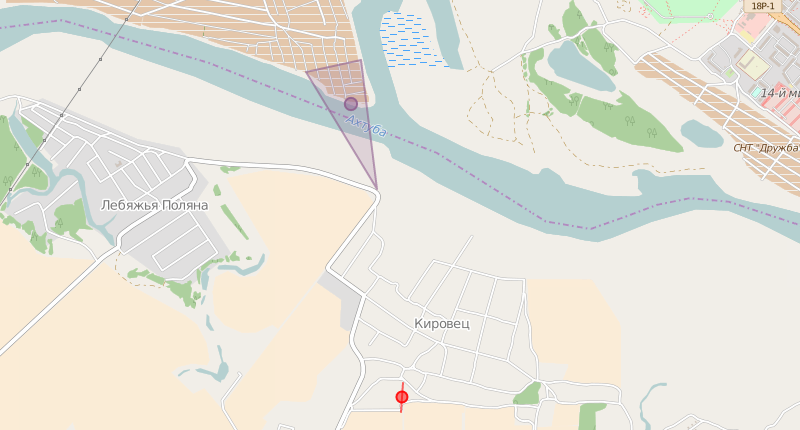
\includegraphics[width=.7\textwidth]{river_surface}\\[1ex]
    \parbox{.9\textwidth}{\caption{Кластеризация выборки из тестового примера <<Река>> с метрикой \emph{Surface}} \label{img:river-sur}}
    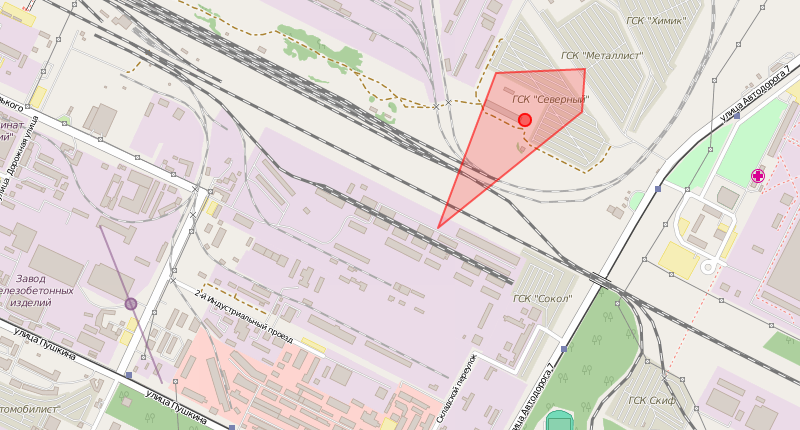
\includegraphics[width=.7\textwidth]{railway_surface}\\[1ex]
    \parbox{.9\textwidth}{\caption{Кластеризация выборки из тестового примера <<Железная дорога>> с метрикой \emph{Surface}} \label{img:railway-sur}}
\end{figure}

Предлагается два способа расчета расстояний между географическими объектами. Первый способ заключается в использовании в качестве расстояний решения обратной геодезической задачи для рассматриваемых точек (метрика <<Surface>>). Второй способ заключается в использовании в качестве расстояний длину маршрута между двумя рассматриваемыми точками (метрика <<Route>>).

\textbf{В третье главе} описана методология проектирования ПО, разработана методика проведения эксперимента, произведено испытание разработанных алгоритмов, а также обсуждены полученные результаты в ходе эксперимента и сделан вывод на их основе.

Предложенные алгоритмы были реализованы с использованием языка программирования Python и сервиса построения маршрутов Open Source Routing Machine (OSRM) для расчета расстояния между географическими точками по городским дорогам.

\begin{figure}[b!]
    \centering
    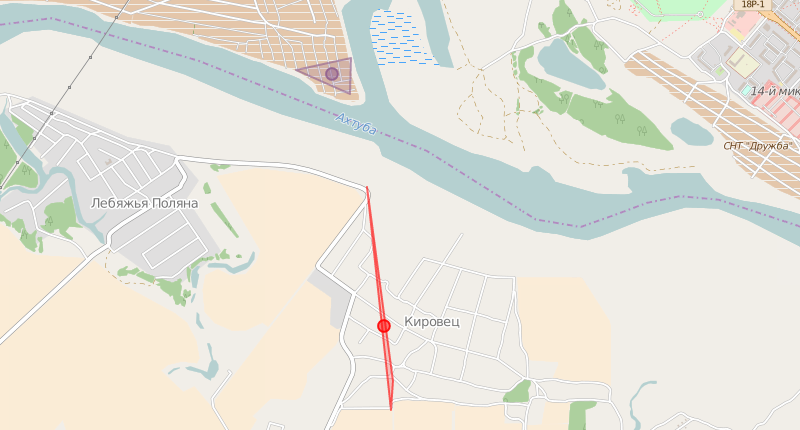
\includegraphics[width=.7\textwidth]{river_route}\\[1ex]
    \parbox{.9\textwidth}{\caption{Кластеризация выборки из тестового примера <<Река>> с метрикой <<Route>>} \label{img:river-route}}
    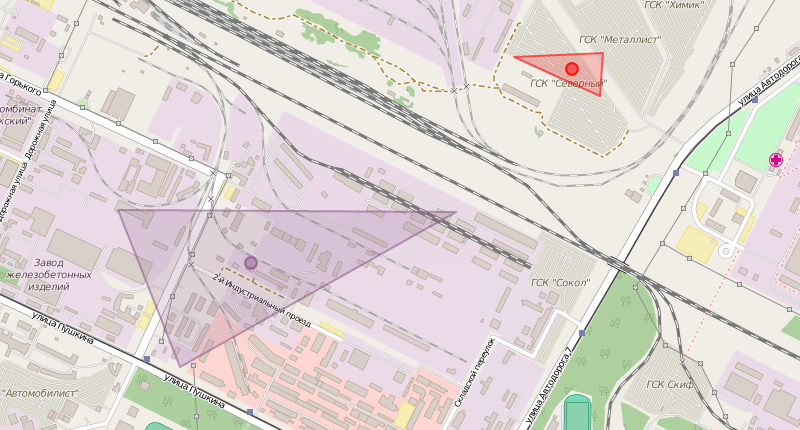
\includegraphics[width=.7\textwidth]{railway_route}\\[1ex]
    \parbox{.9\textwidth}{\caption{Кластеризация выборки из тестового примера <<Железная дорога>> с метрикой <<Route>>} \label{img:railway-route}}
\end{figure}

В качестве тестовых примеров для проверки расчета расстояний было сделано две тестовые выборки: <<Река>>, представленная на рис.~\ref{img:river}, и <<Железная дорога>>, представленная на рис.~\ref{img:railway}, между объектами которых располагаются река и железная дорога соответственно.

При кластеризации выборок из этих примеров с использованием обычных метрик объекты, между которыми находится препятствие, попадают в один кластер: рис.~\ref{img:river-sur}, \ref{img:railway-sur}.

При кластеризации выборок из этих примеров с использованием метрики \emph{Route} объекты, разделенные препятствиями, попадают в разные кластеры: рис.~\ref{img:river-route}, \ref{img:railway-route}.
\begin{figure}[b!]
    \centering
    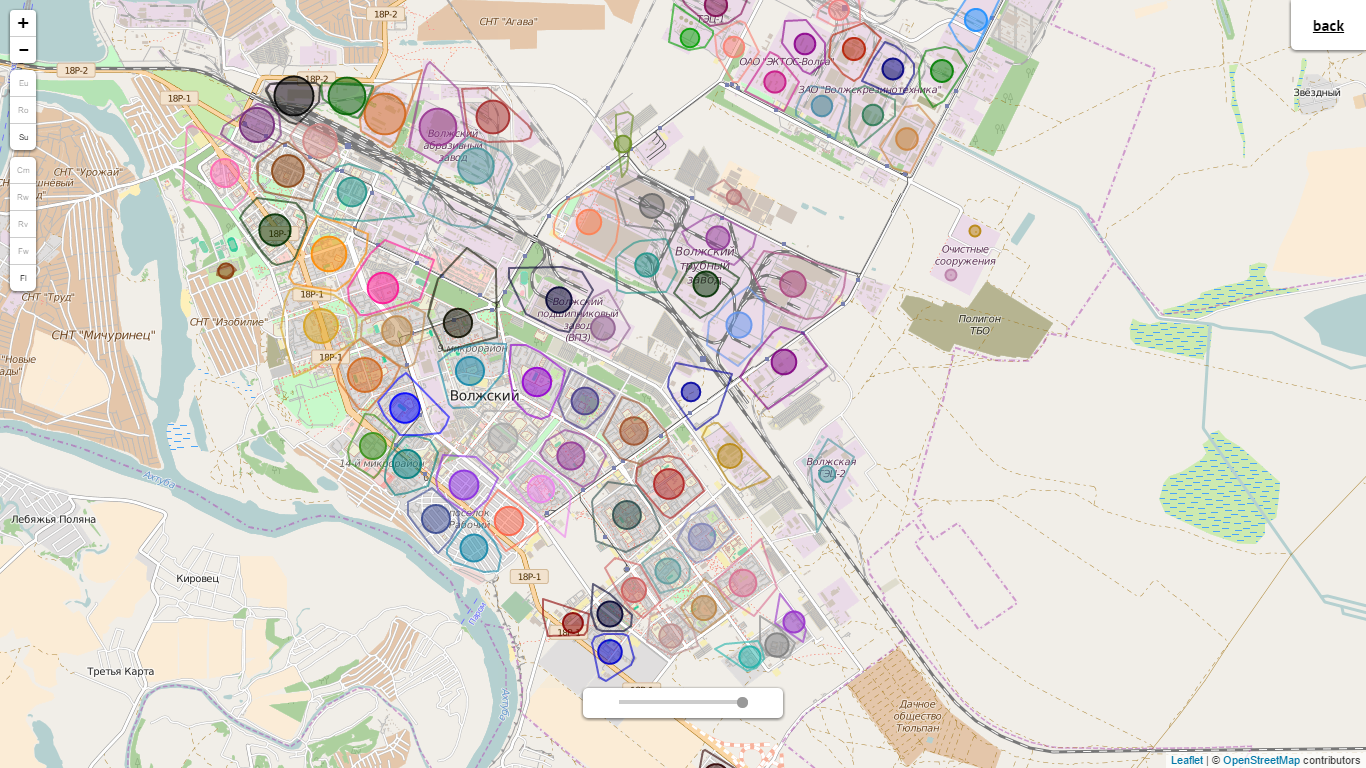
\includegraphics[width=.7\textwidth]{full_surface}\\[1ex]
    \parbox{.9\textwidth}{\caption{Кластеризация выборки \emph{Main} с метрикой \emph{Surface}. Линиями очерчена выпуклая оболочка точек, принадлежащих кластерам. Круги~--- центры кластеров, радиус круга зависит от количества точек, принадлежащих кластеру.} \label{img:full-surface}}
    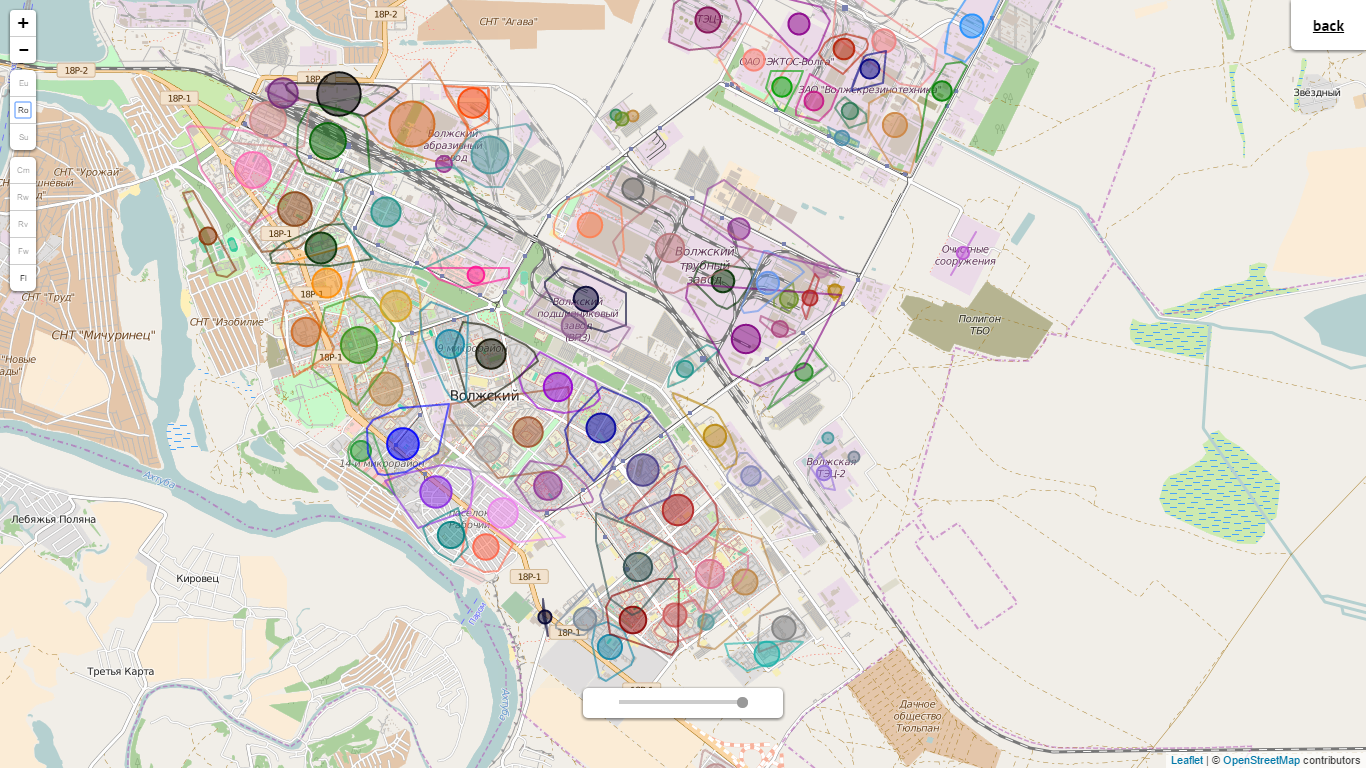
\includegraphics[width=.7\textwidth]{full_route}\\[1ex]
    \parbox{.9\textwidth}{\caption{Кластеризация выборки \emph{Main} с метрикой \emph{Route}. Линиями очерчена выпуклая оболочка точек, принадлежащих кластерам. Круги~--- центры кластеров, радиус круга зависит от количества точек, принадлежащих кластеру.} \label{img:full-route}}
\end{figure}

Метрика \emph{Route} построена на получении данных о расстоянии между точками по графу городской дорожной сети. Для получения этих данных используется сервис построения маршрутов Open Source Routing Machine с профилем работы для автомобиля.

Для тестирования работы алгоритма и метрик была сгенерирована псевдореалистичная выборка данных (<<Main>>), состоящая из 12 тысяч точек. Кластеризация проводилась с идентичным начальным набором из 125 кластеров. Результаты работы представлены на рис.~\ref{img:full-surface}, \ref{img:full-route}. На рисунке~\ref{img:full-route} видно, что области, ограниченные линиями пересекаются. Это происходит из-за того, что при расчете расстояния сервис OSRM выбирает ближайшие к точкам участки дорожной сети, а затем строит маршрут по графу дорог между ними. Из-за этого точки, расположенные, например, по разные стороны одного дома попадают на разные участки дорог, и расстояние между ними и центром кластера получается различным.

Для тестирования работы алгоритма расстановки остановочных пунктов использовалась часть выборки \emph{Main}, детальный вид представлен на рис.~\ref{img:terminals}. Видно, что центры кластеров располагаются на участках дорожной сети.
\begin{figure}[h!]
    \centering
    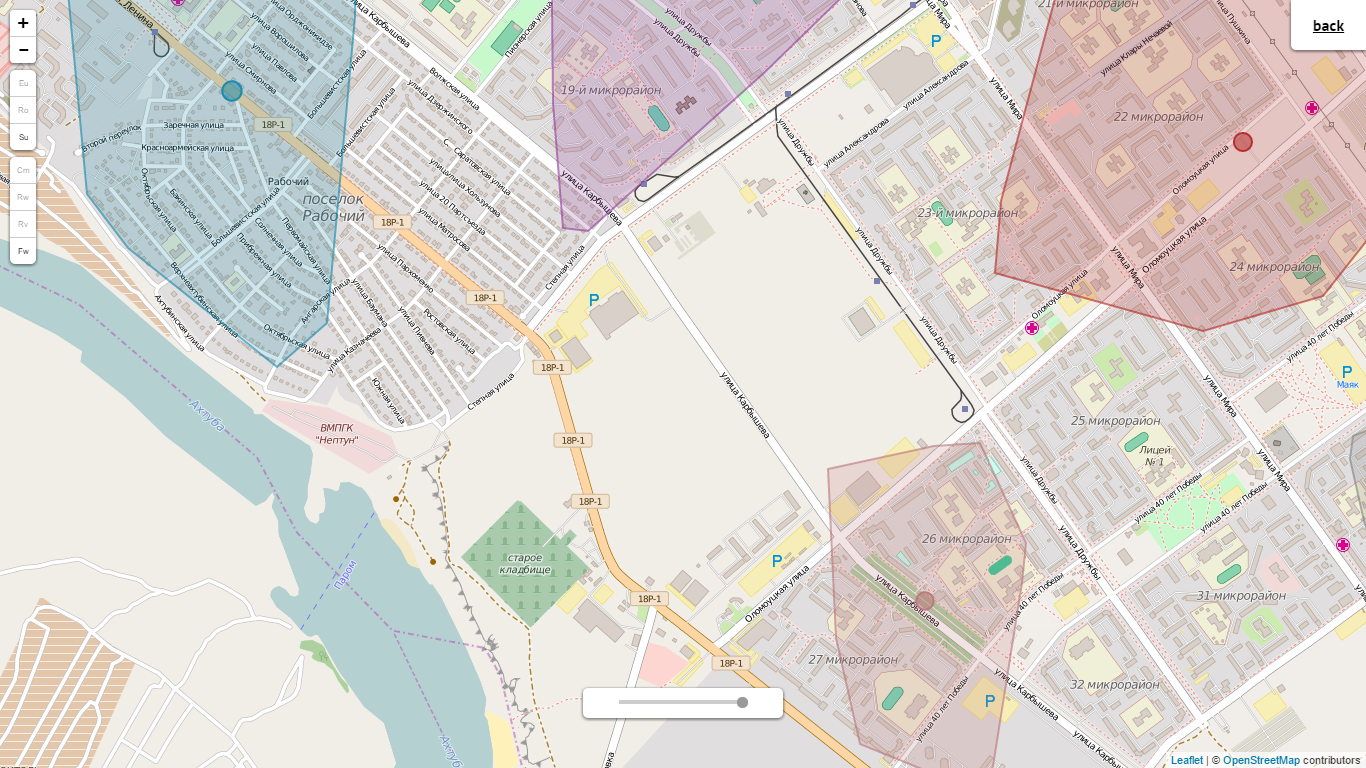
\includegraphics[width=.7\textwidth]{terminals}\\[1ex]
    \parbox{.9\textwidth}{\caption{Пример нахождения остановочных пунктов. Центры кластеров выделены кругами.} \label{img:terminals}}
\end{figure}

\textbf{В четвертой главе} произведена оценка эффективности разработанных алгоритмов, были проведены эксперименты, в ходе которых менялись тестовые выборки, метрики расстояния, а также реализации данного метода.

Кластеризация выборки \emph{Main} (1,5 млн расчетов дистанций) с метрикой \emph{Surface} потребовала 28 итераций алгоритма. При использовании параллельной реализации (4 потока) на одну итерацию в среднем уходит по 17 минут. Кластеризация выборки \emph{Main} с метрикой \emph{Routes} потребовала 21 итерацию алгоритма. При использовании параллельной реализации (4 потока) на одну итерацию в среднем уходит по 90 минут. Откуда можно сделать вывод, что на один расчет расстояния (при параллельной реализации) метрикой \emph{Surface} уходит \( 0.66 \)~мсек, тогда как у метрики \emph{Route} на это затрачивается \( 3.6 \)~мсек. Для сравнения, на один расчет Эвклидовой метрикой уходит \( 0.06 \)~мсек.

При непараллельной версии работы у метрики \emph{Surface} в среднем на один расчет расстояния затрачивается \( 0.71 \)~мсек, у метрики \emph{Route}~--- \( 4.8 \)~мсек. Для сравнения, на один расчет Эвклидовой метрикой уходит \( 0.07 \)~мсек.

\textbf{В заключении} работы сформулированы общие выводы по проделанной работе в рамках магистерской диссертации. Обсуждены полученные результаты и предложено направление для дальнейшего развития данной работы.

\textbf{В приложении} приведены материалы справочного, иллюстративного характера и техническое задание на создание программы формирования маршрутов общественного транспорта на основании обработки данных.

% TODO
\section{Основные результаты работы}
\begin{itemize}
    \item \ldots
\end{itemize}

\section{Перспективные направления развития работы}
Предложенный алгоритм может быть использован для построения сети остановочных пунктов общественного транспорта.
Разработанный модуль может быть использован как компонент системы формирования маршрутной сети городского транспорта.

\renewcommand{\bibname}{Публикации по теме диссертации}
\begin{thebibliography}{10}
    \bibitem{first} Strategway: web solutions for building public transportation routes using big geodata 
        analysis / Golubev A., Chechetkin I., Solnushkin K.S., Sadovnikova N., Parygin D., Shcherbakov M., 
        Brebels A. // Proceedings of The 17th International Conference on Information Integration and 
        Web-based Applications \& Services (iiWAS2015) (December 11 - 13, 2015 Brussels, Belgium) 
        ACM New York, New York pp. 665 - 668
    \bibitem{second} Комплекс инструментов интеллектуального анализа данных strategway для поддержки 
        принятия решений по управлению развитием инфраструктуры города / Садовникова Н.П., Щербаков М.В., 
        Парыгин Д.С., Солнушкин К.С., Голубев А.В., Чечеткин И.А. // В сборнике: Развитие средних 
        городов: замысел, модели, практика Материалы III Международной научно-практической конференции. 
        Волгоград, 2015. С. 147-150
    \bibitem{third} Автоматизация поддержки принятия решений по разработке маршрутов общественного 
        транспорта на основе анализа данных о корреспонденциях жителей / М. В. Щербаков, 
        Н. П. Садовникова, Д. С. Парыгин, А. В. Голубев, И. А. Чечеткин // Вестник компьютерных и 
        информационных технологий. -- М. : Издательский дом <<Спектр>>, 2016. -- В печати.
\end{thebibliography}